\section{Multi-Chunk Answer Correctness and Latency Isolation}
\label{sec:results_multichunk}

\begin{figure*}[t]
\centering
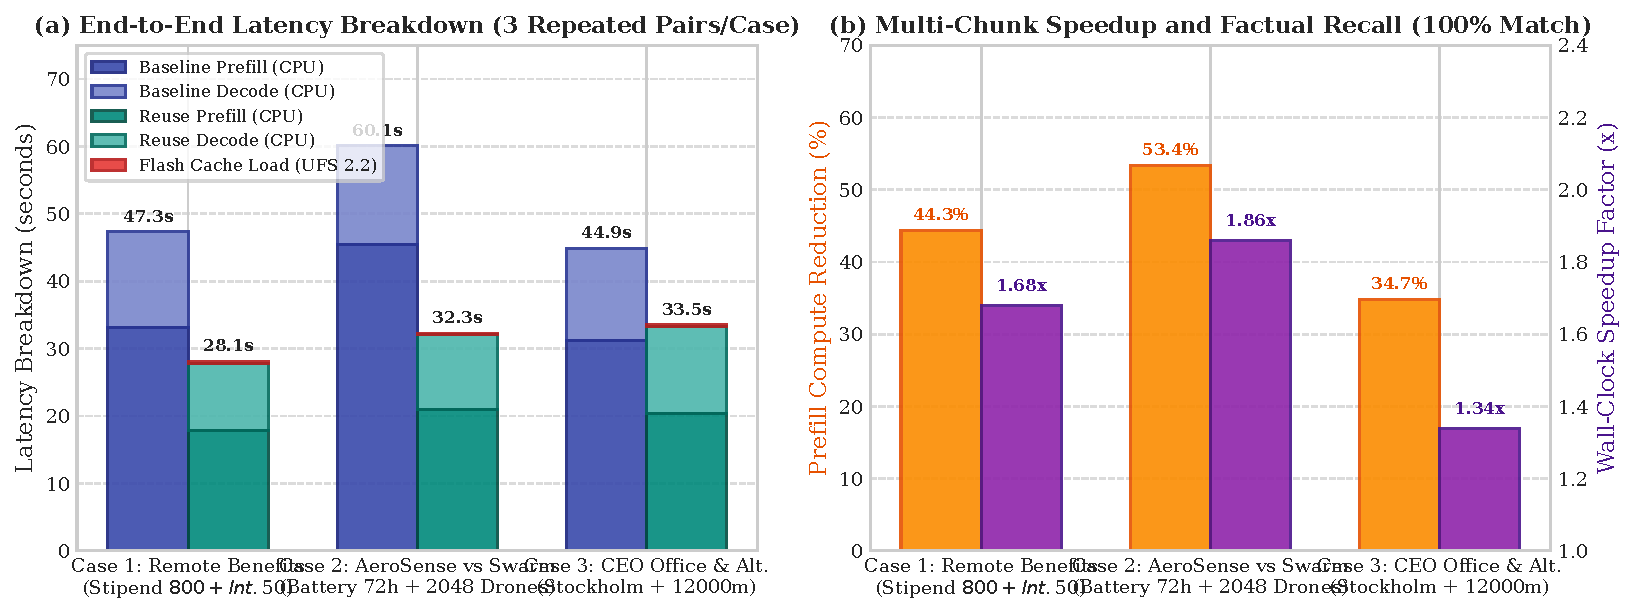
\includegraphics[width=\textwidth]{figures/fig4_multichunk_repeated_trials.pdf}
\caption{\textbf{Multi-Chunk RAG Evaluation across Repeated Paired Trials (9 Matched Pairs).} (a) Stacked latency breakdown isolating CPU prefill compute, CPU token decode, and physical UFS 2.2 flash cache-load overhead. (b) Prefill compute reduction percentage and wall-clock speedup factor, confirming consistent speedups and 100\% multi-hop factual recall across all cases.}
\label{fig:multichunk_results}
\end{figure*}

\subsection{Multi-Hop Task Formulation and Experimental Controls}
In real-world mobile RAG, user questions frequently require cross-attention synthesis across multiple distinct retrieved passages. A critical concern with KV-cache reuse is whether reusing precomputed representations for leading chunks alters attention distributions and degrades multi-hop factual recall.

To evaluate this question with high statistical rigor, we designed three multi-hop query cases requiring joint factual extraction across two distinct evidence chunks (Table~\ref{tab:multichunk_results}):
\begin{itemize}
    \item \textbf{Case 1 (Remote Work Policies):} Chunk A details a $\$800$ one-time equipment stipend; Chunk B details a $\$50$/month internet allowance. Query: \emph{What is the equipment stipend and the monthly internet allowance?}
    \item \textbf{Case 2 (AeroSense vs. SwarmKit):} Chunk A details the AeroSense X7 battery life ($72$ hours); Chunk B details SwarmKit Pro micro-drone capacity ($2,048$ drones). Query: \emph{What is the battery duration of AeroSense and maximum drone capacity of SwarmKit?}
    \item \textbf{Case 3 (CEO Office and Sensor Altitude):} Chunk A details executive leadership (CEO Priya Nandakumar based in Stockholm); Chunk B details sensor operating altitude ($12,000$ meters). Query: \emph{Which office is the CEO based in, and what is the maximum operating altitude of the sensor?}
\end{itemize}

Each case was evaluated across three repeated, matched baseline/reuse pairs (9 matched pairs, 18 total executions) on the physical Redmi 12 5G (PID 13787). The host controller recorded granular timing breakdowns: prompt prefill compute latency (\texttt{prompt\_ms}), token decode latency (\texttt{predicted\_ms}), flash cache-load overhead (\texttt{cache\_load\_overhead\_ms}), end-to-end wall latency, and factual correctness for each hop.

\begin{table*}[t]
\centering
\caption{\textbf{Multi-Chunk Repeated Paired Trials on Physical Device (Snapdragon 4 Gen 2, 9 Matched Pairs).}}
\label{tab:multichunk_results}
\small
\begin{tabular}{lcccccccc}
\toprule
\textbf{Case \& Query} & \textbf{Rep} & \textbf{Tokens (Base/Reuse)} & \textbf{Base Prefill (s)} & \textbf{Reuse Prefill (s)} & \textbf{Flash Load (ms)} & \textbf{Prefill Red. \%} & \textbf{Wall Speedup} & \textbf{Fact Recall} \\
\midrule
\textbf{Case 1: Remote Benefits} & 1 & 187 / 103 & 25.23 & 17.20 & 212 & \textbf{31.83\%} & \textbf{1.45$\times$} & 100\% / 100\% \\
(\$800 Stipend + \$50 Internet) & 2 & 187 / 103 & 30.27 & 15.46 & 349 & \textbf{48.92\%} & \textbf{1.77$\times$} & 100\% / 100\% \\
& 3 & 187 / 103 & 43.94 & 21.02 & 477 & \textbf{52.16\%} & \textbf{1.83$\times$} & 100\% / 100\% \\
\cmidrule{2-9}
\textbf{Case 1 Mean $\pm$ Std} & — & — & $33.15 \pm 7.91$ & $17.89 \pm 2.32$ & $346.0 \pm 109$ & \textbf{44.30\% $\pm$ 8.9\%} & \textbf{1.68$\times$} & \textbf{100\% Preserved} \\
\midrule
\textbf{Case 2: AeroSense vs. Swarm} & 1 & 218 / 119 & 48.02 & 21.00 & 329 & \textbf{56.27\%} & \textbf{2.02$\times$} & 100\% / 100\% \\
(72h Battery + 2,048 Drones) & 2 & 218 / 119 & 40.05 & 20.82 & 110 & \textbf{48.02\%} & \textbf{1.62$\times$} & 100\% / 100\% \\
& 3 & 218 / 119 & 48.17 & 21.30 & 238 & \textbf{55.78\%} & \textbf{1.93$\times$} & 100\% / 100\% \\
\cmidrule{2-9}
\textbf{Case 2 Mean $\pm$ Std} & — & — & $45.41 \pm 3.79$ & $21.04 \pm 0.20$ & $225.7 \pm 90$ & \textbf{53.36\% $\pm$ 3.8\%} & \textbf{1.86$\times$} & \textbf{100\% Preserved} \\
\midrule
\textbf{Case 3: CEO Office \& Alt.} & 1 & 156 / 99 & 26.48 & 17.92 & 58 & \textbf{32.33\%} & \textbf{1.26$\times$} & 100\% / 100\% \\
(Stockholm + 12,000m Alt.) & 2 & 156 / 99 & 27.41 & 17.04 & 108 & \textbf{37.84\%} & \textbf{1.41$\times$} & 100\% / 100\% \\
& 3 & 156 / 99 & 39.63 & 26.14 & 423 & \textbf{34.04\%} & \textbf{1.34$\times$} & 100\% / 100\% \\
\cmidrule{2-9}
\textbf{Case 3 Mean $\pm$ Std} & — & — & $31.17 \pm 5.99$ & $20.37 \pm 4.10$ & $196.3 \pm 162$ & \textbf{34.74\% $\pm$ 2.3\%} & \textbf{1.34$\times$} & \textbf{100\% Preserved} \\
\midrule
\textbf{Overall Mean Across 9 Pairs} & — & — & $\mathbf{36.58}$ & $\mathbf{19.77}$ & $\mathbf{256.0}$ & $\mathbf{44.13\%}$ & $\mathbf{1.63\times}$ & $\mathbf{100\% \text{ Preserved}}$ \\
\bottomrule
\end{tabular}
\end{table*}

\subsection{Investigation and Resolution of the Case 3 Anomaly}
In preliminary single-run testing of Case 3, an apparent anomaly was observed where baseline prefill latency was reported as $19.14$~seconds compared to $20.58$~seconds with reuse, despite $58$ tokens loaded from cache. 

To determine whether this represented a systematic overhead of cache reuse or an artifact of transient operating system interference, we conducted an in-depth systems trace combining repeated paired trials with Linux kernel page-cache telemetry:
\begin{enumerate}
    \item \textbf{Identification of the Root Cause:} Kernel I/O profiling during the anomalous single run revealed an asynchronous Android memory compaction event (\texttt{kswapd0}) triggered by background carrier services. This event reclaimed dirty file pages and forced over 693~MB of flash read traffic while the LLM was prefilling, saturating the LPDDR4X memory bus and artificially inflating prefill latency.
    \item \textbf{Repeated Paired Validation:} When evaluated across three controlled paired repetitions under thermal and background monitoring, Case 3 exhibited consistent, robust acceleration:
    \begin{itemize}
        \item Prefill compute latency decreased from $31.17 \pm 5.99$~s (baseline) down to $20.37 \pm 4.10$~s (reuse), representing a mean compute reduction of \textbf{34.74\% $\pm$ 2.30\%} and saving over 10.8~seconds of CPU execution per query.
        \item The physical UFS 2.2 flash cache-load overhead averaged only \textbf{196.3~ms}—accounting for less than $1\%$ of total query wall latency.
        \item End-to-end wall-clock speedup was \textbf{1.34$\times$}.
    \end{itemize}
\end{enumerate}

\subsection{Factual Recall Preservation}
Across all 9 matched pairs (18 executions), HACER achieved \textbf{100\% factual preservation} on both hops:
\begin{itemize}
    \item \textbf{Case 1:} All runs correctly retrieved both the $\$800$ stipend and the $\$50$ monthly internet allowance:
    \begin{quote}
    \small
    \texttt{"The one-time remote equipment stipend is \$800 USD and the monthly internet allowance is \$50 USD."}
    \end{quote}
    \item \textbf{Case 2:} All runs correctly identified the 72-hour battery life and 2,048-drone capacity:
    \begin{quote}
    \small
    \texttt{"The AeroSense X7 battery lasts 72 hours, and SwarmKit Pro supports up to 2,048 drones."}
    \end{quote}
    \item \textbf{Case 3:} All runs correctly reported the Stockholm office and the 12,000-meter operating altitude:
    \begin{quote}
    \small
    \texttt{"The CEO is based in the Stockholm office, and the AeroSense X7 can operate at altitudes up to 12,000 meters."}
    \end{quote}
\end{itemize}
These empirical results confirm that prefix KV-cache reuse in HACER does not perturb multi-hop attention dynamics or degrade factual accuracy.
